\documentclass[11pt,a4paper]{article}

% --- PAQUETES DE IDIOMA Y CODIFICACIÓN ---
\usepackage[utf8]{inputenc}
\usepackage[T1]{fontenc}
\usepackage[spanish,es-tabla,es-nodecimaldot,es-noshorthands]{babel}

% --- MATEMÁTICAS Y SÍMBOLOS ---
\usepackage{amsmath,amssymb,amsfonts}
\usepackage{mathtools}

% --- FORMATO Y DISEÑO DE PÁGINA ---
\usepackage[top=2.5cm, bottom=2.5cm, left=2.5cm, right=2.5cm]{geometry}
\usepackage{fancyhdr}
\usepackage{booktabs}
\usepackage{array}
\usepackage{enumitem}
\usepackage{titlesec}
\usepackage{graphicx}

% --- COLORES Y CÓDIGO ---
\usepackage[table]{xcolor}
\definecolor{pujblue}{RGB}{0, 51, 102}
\definecolor{darkblue}{RGB}{16, 44, 87}
\definecolor{codebg}{RGB}{248, 249, 250}
\definecolor{darkgray}{RGB}{60, 60, 60}

\usepackage{listings}
\usepackage[colorlinks=true, linkcolor=pujblue, citecolor=pujblue, urlcolor=pujblue]{hyperref}

% --- CONFIGURACIÓN DE LISTINGS ---
\lstset{
    language=Python,
    backgroundcolor=\color{codebg},
    basicstyle=\ttfamily\footnotesize,
    keywordstyle=\color{pujblue}\bfseries,
    commentstyle=\color{gray}\itshape,
    stringstyle=\color{teal},
    breaklines=true,
    frame=single,
    rulecolor=\color{black!20},
    numbers=left,
    numberstyle=\tiny\color{gray},
    numbersep=8pt,
    tabsize=4,
    showstringspaces=false,
    literate=
      {á}{{\'a}}1 {é}{{\'e}}1 {í}{{\'i}}1 {ó}{{\'o}}1 {ú}{{\'u}}1
      {Á}{{\'A}}1 {É}{{\'E}}1 {Í}{{\'I}}1 {Ó}{{\'O}}1 {Ú}{{\'U}}1
      {ñ}{{\~n}}1 {Ñ}{{\~N}}1 {ü}{{\"u}}1 {Ü}{{\"U}}1
      {¿}{{?`}}1 {¡}{{!`}}1
}

% --- ENCABEZADOS Y PIES DE PÁGINA ---
\pagestyle{fancy}
\fancyhf{}
\fancyhead[L]{\small\color{darkgray}\textit{Computación Científica}}
\fancyhead[R]{\small\color{darkgray}\textit{Taller de Búsqueda de Raíces}}
\fancyfoot[C]{\thepage}
\renewcommand{\headrulewidth}{0.4pt}
\renewcommand{\footrulewidth}{0.4pt}

\titleformat{\section}{\Large\bfseries\color{pujblue}}{\thesection}{1em}{}[\titlerule]
\titleformat{\subsection}{\large\bfseries\color{darkblue}}{\thesubsection}{1em}{}
\titleformat{\subsubsection}{\normalsize\bfseries\color{darkblue}}{\thesubsubsection}{1em}{}

% ==============================================================================
% INICIO DEL DOCUMENTO
% ==============================================================================
\begin{document}

\begin{center}
    {\LARGE\bfseries\color{pujblue} Taller de Búsqueda de Raíces}\\[0.3cm]
    {\large Computación Científica --- Pontificia Universidad Javeriana Cali}\\[0.1cm]
    {\normalsize Profesor: Juan Fernando Paz}\\[0.1cm]
    {\normalsize Estudiante: Miguel Angel Padilla Rosero}
\end{center}
\vspace{0.3cm}

% ==============================================================================
% CÓDIGO BASE EN PYTHON
% ==============================================================================
\section{Implementación de los Algoritmos Base en Python}

Para resolver el taller se implementaron los cinco métodos numéricos en Python. Siguiendo una estructura limpia, los ciclos se controlan mediante banderas (\textit{flags}) y condicionales, usando un único punto de retorno al final y evitando sentencias como \texttt{break} o \texttt{continue}:

\begin{lstlisting}
import numpy as np

def biseccion(f, a, b, tol, max_iter=200):
    iters = 0
    terminado = False
    while not terminado and iters < max_iter:
        error = (b - a) / 2.0
        if error < tol:
            terminado = True
        else:
            iters += 1
            m = (a + b) / 2.0
            if f(a) * f(m) <= 0:
                b = m
            else:
                a = m
    raiz = (a + b) / 2.0
    return raiz, iters

def newton_raphson(f, df, x0, tol, max_iter=200):
    iters = 0
    x = x0
    terminado = False
    while not terminado and iters < max_iter:
        iters += 1
        x_next = x - f(x) / df(x)
        error = abs(x_next - x)
        if error < tol:
            terminado = True
        x = x_next
    return x, iters

def secante(f, x0, x1, tol, max_iter=200):
    iters = 0
    terminado = False
    p0 = x0
    p1 = x1
    raiz = p1
    while not terminado and iters < max_iter:
        iters += 1
        fp0 = f(p0)
        fp1 = f(p1)
        p2 = p1 - fp1 * (p1 - p0) / (fp1 - fp0)
        error = abs(p2 - p1)
        if error < tol:
            terminado = True
        p0 = p1
        p1 = p2
        raiz = p2
    return raiz, iters

def falsa_posicion(f, a, b, tol, max_iter=200):
    iters = 0
    terminado = False
    c_prev = None
    raiz = a
    while not terminado and iters < max_iter:
        iters += 1
        fa = f(a)
        fb = f(b)
        c = b - fb * (b - a) / (fb - fa)
        fc = f(c)
        if c_prev is not None and abs(c - c_prev) < tol:
            terminado = True
        else:
            c_prev = c
            if fa * fc <= 0:
                b = c
            else:
                a = c
        raiz = c
    return raiz, iters

def punto_fijo(g, x0, tol, max_iter=200):
    iters = 0
    x = x0
    terminado = False
    while not terminado and iters < max_iter:
        iters += 1
        x_next = g(x)
        error = abs(x_next - x)
        if error < tol:
            terminado = True
        x = x_next
    return x, iters
\end{lstlisting}

% ==============================================================================
% ACTIVIDAD 1
% ==============================================================================
\section{Actividad 1: Un problema de laboratorio}

Durante un experimento de laboratorio se midió la temperatura $T$ de una muestra en diferentes instantes de tiempo $t$:

\begin{table}[h!]
    \centering
    \caption{Datos experimentales de temperatura vs. tiempo.}
    \begin{tabular}{ccccccc}
        \toprule
        $t$ [min] & $0$ & $1$ & $2$ & $3$ & $4$ & $5$ \\
        \midrule
        $T$ [$^\circ$C] & $21.0$ & $23.8$ & $28.1$ & $34.5$ & $43.2$ & $55.0$ \\
        \bottomrule
    \end{tabular}
\end{table}

El objetivo es determinar en qué instante la muestra alcanza la temperatura crítica de $T_{\text{crit}} = 60^\circ\text{C}$ para detener el proceso.

\subsection{Construcción de la función $T(t)$}
Como tenemos 6 datos con tiempos diferentes, usamos el polinomio interpolante. Por el teorema de interpolación, existe un único polinomio de grado menor o igual a 5 que pasa por todos los puntos:
\begin{equation}
    T(t) = c_0 + c_1 t + c_2 t^2 + c_3 t^3 + c_4 t^4 + c_5 t^5
\end{equation}

Para hallar los coeficientes, se evalúa el polinomio en cada instante medido ($T(t_i) = T_i$ para $i=0,\dots,5$). Esto nos deja el sistema matricial $V c = T$, donde $V$ es la matriz de Vandermonde:
\begin{equation}
    \begin{pmatrix}
        1 & 0 & 0 & 0 & 0 & 0 \\
        1 & 1 & 1 & 1 & 1 & 1 \\
        1 & 2 & 4 & 8 & 16 & 32 \\
        1 & 3 & 9 & 27 & 81 & 243 \\
        1 & 4 & 16 & 64 & 256 & 1024 \\
        1 & 5 & 25 & 125 & 625 & 3125
    \end{pmatrix}
    \begin{pmatrix}
        c_0 \\ c_1 \\ c_2 \\ c_3 \\ c_4 \\ c_5
    \end{pmatrix}
    =
    \begin{pmatrix}
        21.0 \\ 23.8 \\ 28.1 \\ 34.5 \\ 43.2 \\ 55.0
    \end{pmatrix}
\end{equation}

Como los tiempos son todos diferentes, el determinante de $V$ es distinto de cero y el sistema tiene solución única. Resolviendo el sistema en Python obtenemos los coeficientes:
\begin{equation}
    c_0 = 21, \quad c_1 = 2.55, \quad c_2 = -0.15, \quad c_3 = \frac{59}{120} \approx 0.491667, \quad c_4 = -0.1, \quad c_5 = \frac{1}{120} \approx 0.008333
\end{equation}

Por lo tanto, la función de temperatura es:
\begin{equation}
    T(t) = 21 + 2.55\,t - 0.15\,t^2 + 0.491667\,t^3 - 0.1\,t^4 + 0.008333\,t^5
\end{equation}

Para verificar, evaluamos el polinomio en algunos datos:
\begin{align*}
    T(0) &= 21.0^\circ\text{C} \\
    T(1) &= 21 + 2.55 - 0.15 + 0.491667 - 0.1 + 0.008333 = 23.8^\circ\text{C} \\
    T(5) &= 21 + 12.75 - 3.75 + 61.458333 - 62.5 + 26.041667 = 55.0^\circ\text{C}
\end{align*}
lo que coincide de forma exacta con la tabla experimental.

\subsection{Búsqueda del instante en que se alcanza la temperatura crítica}
Buscamos el tiempo $t$ tal que $T(t) = 60^\circ\text{C}$. Restando 60 a ambos lados, definimos la función $f(t) = 0$:
\begin{equation}
    f(t) = T(t) - 60 = 0.008333\,t^5 - 0.1\,t^4 + 0.491667\,t^3 - 0.15\,t^2 + 2.55\,t - 39
\end{equation}

Derivando término a término obtenemos $f'(t)$, necesaria para Newton-Raphson:
\begin{equation}
    f'(t) = 0.041667\,t^4 - 0.4\,t^3 + 1.475\,t^2 - 0.3\,t + 2.55
\end{equation}

\paragraph{Intervalo inicial y unicidad:}
En $t = 5\text{ min}$, la muestra está a $55^\circ\text{C}$, por lo que:
\begin{equation}
    f(5) = 55 - 60 = -5 < 0
\end{equation}
Si evaluamos el polinomio en $t = 6\text{ min}$:
\begin{equation}
    T(6) = 72.3^\circ\text{C} \implies f(6) = 72.3 - 60 = 12.3 > 0
\end{equation}
Como $f$ es continua y cambia de signo en $[5, 6]$, por el Teorema del Valor Intermedio existe al menos una raíz en ese intervalo. Además, evaluando la derivada se tiene $f'(5) \approx 13.97 > 0$ y $f'(6) \approx 21.45 > 0$, y se verifica que $f'(t) > 0$ en todo $[5, 6]$. Por lo tanto, la función es estrictamente creciente y la raíz es única.

\subsection{Desarrollo de los métodos}
Usamos el intervalo $[5, 6]$ para bisección y secante, y $t_0 = 5$ para Newton-Raphson.

\begin{itemize}[leftmargin=*]
    \item \textbf{Bisección:} Calcula el punto medio $c_k = \frac{a_k + b_k}{2}$ y conserva el subintervalo donde hay cambio de signo. Como el intervalo se reduce a la mitad en cada paso, después de $k$ iteraciones el semiancho mide $\frac{1}{2^{k+1}}$, lo que permite saber con certeza que se cumple la tolerancia cuando $k > \log_2(1/\varepsilon) - 1$.
    \begin{table}[h!]
        \centering
        \caption{Primeras cuatro iteraciones de Bisección (Actividad 1).}
        \begin{tabular}{ccccc}
            \toprule
            $k$ & $a_k$ & $b_k$ & $c_k$ & $f(c_k)$ \\
            \midrule
            $1$ & $5.000000$ & $6.000000$ & $5.500000$ & $2.722656$ \\
            $2$ & $5.000000$ & $5.500000$ & $5.250000$ & $-1.333813$ \\
            $3$ & $5.250000$ & $5.500000$ & $5.375000$ & $0.641511$ \\
            $4$ & $5.250000$ & $5.375000$ & $5.312500$ & $-0.358836$ \\
            \bottomrule
        \end{tabular}
    \end{table}

    \item \textbf{Newton-Raphson:} Usa la recta tangente $t_{k+1} = t_k - \frac{f(t_k)}{f'(t_k)}$. Empezando en $t_0 = 5$:
    \begin{equation}
        t_1 = 5 - \frac{-5.0}{13.966667} \approx 5.357995
    \end{equation}
    \begin{table}[h!]
        \centering
        \caption{Iteraciones de Newton-Raphson (Actividad 1).}
        \begin{tabular}{ccccc}
            \toprule
            $k$ & $t_k$ & $f(t_k)$ & $f'(t_k)$ & $t_{k+1}$ \\
            \midrule
            $0$ & $5.000000$ & $-5.000000$ & $13.966667$ & $5.357995$ \\
            $1$ & $5.357995$ & $0.366767$ & $16.099718$ & $5.335214$ \\
            $2$ & $5.335214$ & $0.001728$ & $15.948400$ & $5.335106$ \\
            \bottomrule
        \end{tabular}
    \end{table}

    \item \textbf{Secante:} Reemplaza la derivada por la pendiente de la recta secante con $t_0 = 5$ y $t_1 = 6$:
    \begin{equation}
        t_2 = 6 - 12.3 \cdot \frac{6 - 5}{12.3 - (-5.0)} = 6 - \frac{12.3}{17.3} \approx 5.289017
    \end{equation}
    \begin{table}[h!]
        \centering
        \caption{Iteraciones de la Secante (Actividad 1).}
        \begin{tabular}{ccccc}
            \toprule
            $k$ & $t_{k-1}$ & $t_k$ & $f(t_k)$ & $t_{k+1}$ \\
            \midrule
            $1$ & $5.000000$ & $6.000000$ & $12.300000$ & $5.289017$ \\
            $2$ & $6.000000$ & $5.289017$ & $-0.728076$ & $5.328751$ \\
            $3$ & $5.289017$ & $5.328751$ & $-0.101218$ & $5.335166$ \\
            $4$ & $5.328751$ & $5.335166$ & $0.000965$ & $5.335106$ \\
            \bottomrule
        \end{tabular}
    \end{table}
\end{itemize}

\subsection{Resultado}
Los métodos convergen al valor:
\begin{equation}
    t^* \approx 5.335106\text{ min}
\end{equation}
Es decir, aproximadamente a los \textbf{5 minutos y 20 segundos} la muestra alcanza la temperatura crítica de $60^\circ\text{C}$ y el calentamiento debe detenerse.

\begin{figure}[h!]
    \centering
    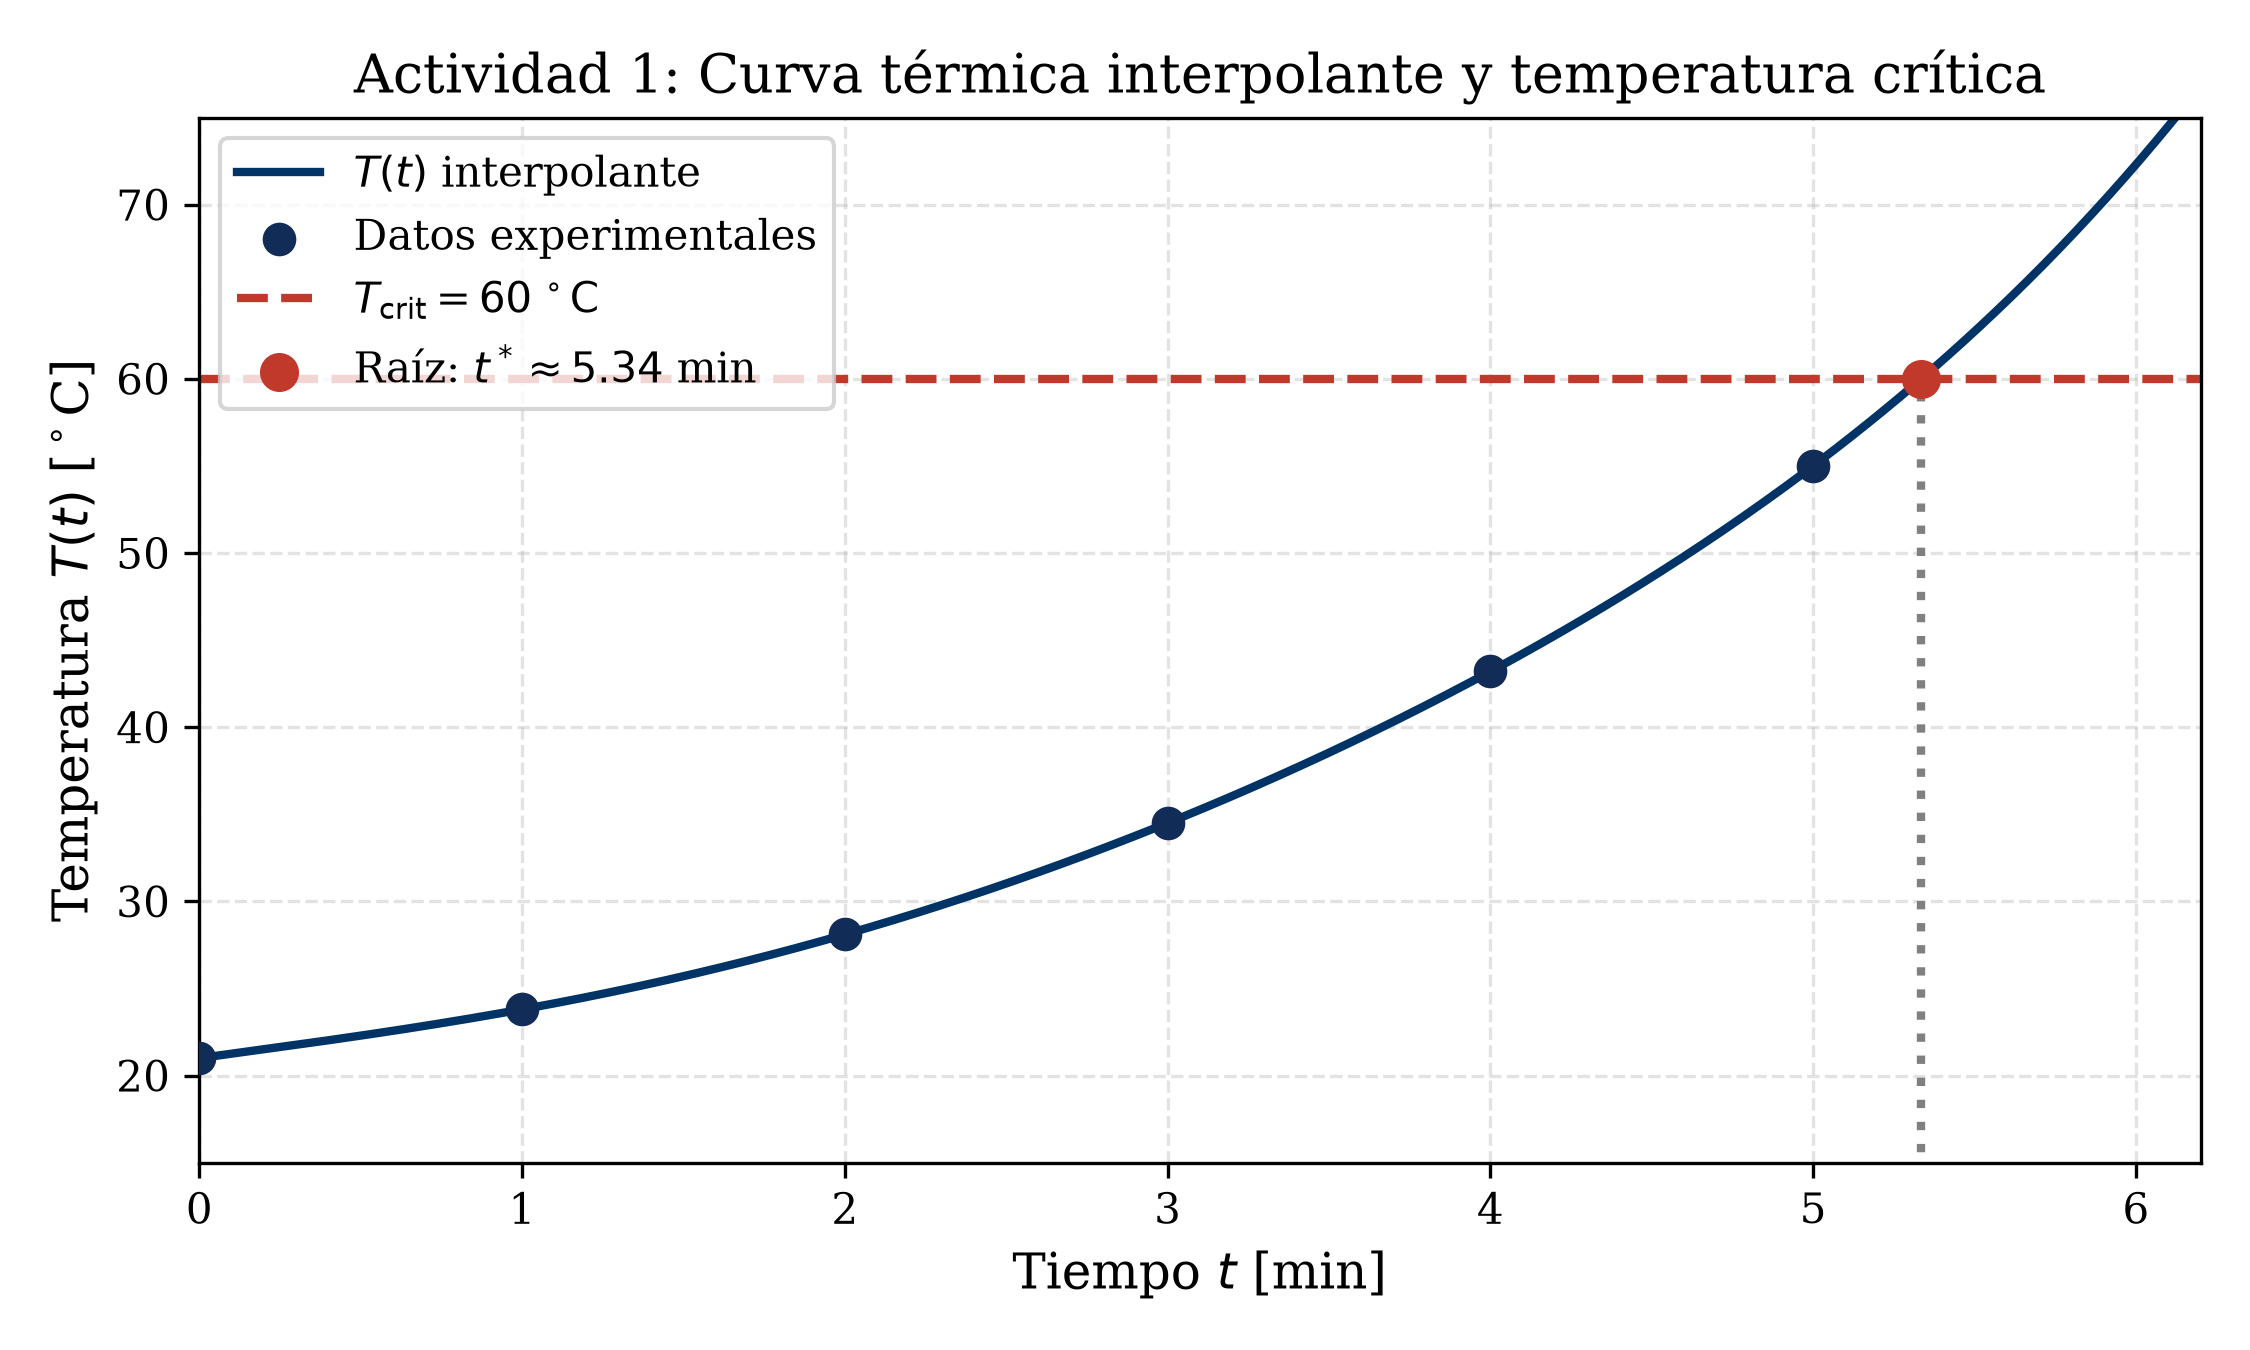
\includegraphics[width=0.72\textwidth]{fig_actividad1_polinomio_temperatura.png}
    \caption{Curva $T(t)$, puntos de laboratorio y ubicación del instante crítico $t^*$.}
\end{figure}

% ==============================================================================
% ACTIVIDAD 2
% ==============================================================================
\section{Actividad 2: Un problema de Ingeniería de Sistemas}

Un servicio dentro de un sistema distribuido tiene un tiempo de respuesta en milisegundos que depende del tamaño de la entrada $n$:
\begin{equation}
    T(n) = 0.02\,n\log_2(n) + 0.5\,e^{0.003\,n}
\end{equation}

El servicio tiene un presupuesto máximo de $100\text{ ms}$. Se pide hallar el tamaño máximo de entrada $n$ que puede procesarse sin exceder ese tiempo.

\subsection{Planteamiento y derivada}
Buscamos el punto de corte con el límite permitido, $T(n) = 100$, lo que equivale a resolver $f(n) = 0$:
\begin{equation}
    f(n) = 0.02\,n\log_2(n) + 0.5\,e^{0.003\,n} - 100 = 0
\end{equation}

Teniendo en cuenta que $\log_2(n) = \frac{\ln(n)}{\ln(2)}$, derivamos la función para aplicar Newton:
\begin{equation}
    f'(n) = 0.02\left(\log_2(n) + \frac{1}{\ln(2)}\right) + 0.0015\,e^{0.003\,n}
\end{equation}

\paragraph{Intervalo inicial y unicidad:}
Evaluando en algunos valores de prueba:
\begin{align*}
    f(500) &= 0.02(500)\log_2(500) + 0.5\,e^{1.5} - 100 \approx -8.101313 < 0 \\
    f(600) &= 0.02(600)\log_2(600) + 0.5\,e^{1.8} - 100 \approx +13.770648 > 0
\end{align*}
Como $f(500) < 0$ y $f(600) > 0$, y la función es continua para $n > 0$, el Teorema del Valor Intermedio asegura una raíz en $[500, 600]$. Como $f'(n) > 0$ para todo $n \ge 1$, la función siempre es creciente y la raíz es única.

\subsection{Desarrollo de los métodos}
\begin{itemize}[leftmargin=*]
    \item \textbf{Bisección:} Comienza en $[500, 600]$ (longitud inicial 100).
    \begin{table}[h!]
        \centering
        \caption{Primeras cuatro iteraciones de Bisección (Actividad 2).}
        \begin{tabular}{ccccc}
            \toprule
            $k$ & $a_k$ & $b_k$ & $c_k$ & $f(c_k)$ \\
            \midrule
            $1$ & $500.000000$ & $600.000000$ & $550.000000$ & $2.739656$ \\
            $2$ & $500.000000$ & $550.000000$ & $525.000000$ & $-2.704806$ \\
            $3$ & $525.000000$ & $550.000000$ & $537.500000$ & $0.011467$ \\
            $4$ & $525.000000$ & $537.500000$ & $531.250000$ & $-1.348163$ \\
            \bottomrule
        \end{tabular}
    \end{table}

    \item \textbf{Newton-Raphson:} Empezando en $n_0 = 500$, con $f(500) \approx -8.101313$ y $f'(500) \approx 0.214892$:
    \begin{equation}
        n_1 = 500 - \frac{-8.101313}{0.214892} \approx 537.699440
    \end{equation}
    \begin{table}[h!]
        \centering
        \caption{Iteraciones de Newton-Raphson (Actividad 2).}
        \begin{tabular}{ccccc}
            \toprule
            $k$ & $n_k$ & $f(n_k)$ & $f'(n_k)$ & $n_{k+1}$ \\
            \midrule
            $0$ & $500.000000$ & $-8.101313$ & $0.214892$ & $537.699440$ \\
            $1$ & $537.699440$ & $0.054903$ & $0.217795$ & $537.447356$ \\
            $2$ & $537.447356$ & $0.000002$ & $0.217775$ & $537.447345$ \\
            \bottomrule
        \end{tabular}
    \end{table}

    \item \textbf{Secante:} Con $n_0 = 500$ y $n_1 = 600$:
    \begin{table}[h!]
        \centering
        \caption{Iteraciones de la Secante (Actividad 2).}
        \begin{tabular}{ccccc}
            \toprule
            $k$ & $n_{k-1}$ & $n_k$ & $f(n_k)$ & $n_{k+1}$ \\
            \midrule
            $1$ & $500.000000$ & $600.000000$ & $13.770648$ & $537.039718$ \\
            $2$ & $600.000000$ & $537.039718$ & $-0.088765$ & $537.442957$ \\
            $3$ & $537.039718$ & $537.442957$ & $-0.000956$ & $537.447345$ \\
            \bottomrule
        \end{tabular}
    \end{table}
\end{itemize}

\subsection{Resultado}
La raíz continua es $n^* \approx 537.447345$. Como la entrada debe ser un número entero y no se puede superar el límite de $100\text{ ms}$, evaluamos los dos enteros vecinos:
\begin{align}
    T(537) &\approx 99.90\text{ ms} < 100\text{ ms} \\
    T(538) &\approx 100.12\text{ ms} > 100\text{ ms}
\end{align}
Por lo tanto, el tamaño máximo de entrada permitido es:
\begin{equation}
    \boxed{n_{\max} = 537}
\end{equation}

\begin{figure}[h!]
    \centering
    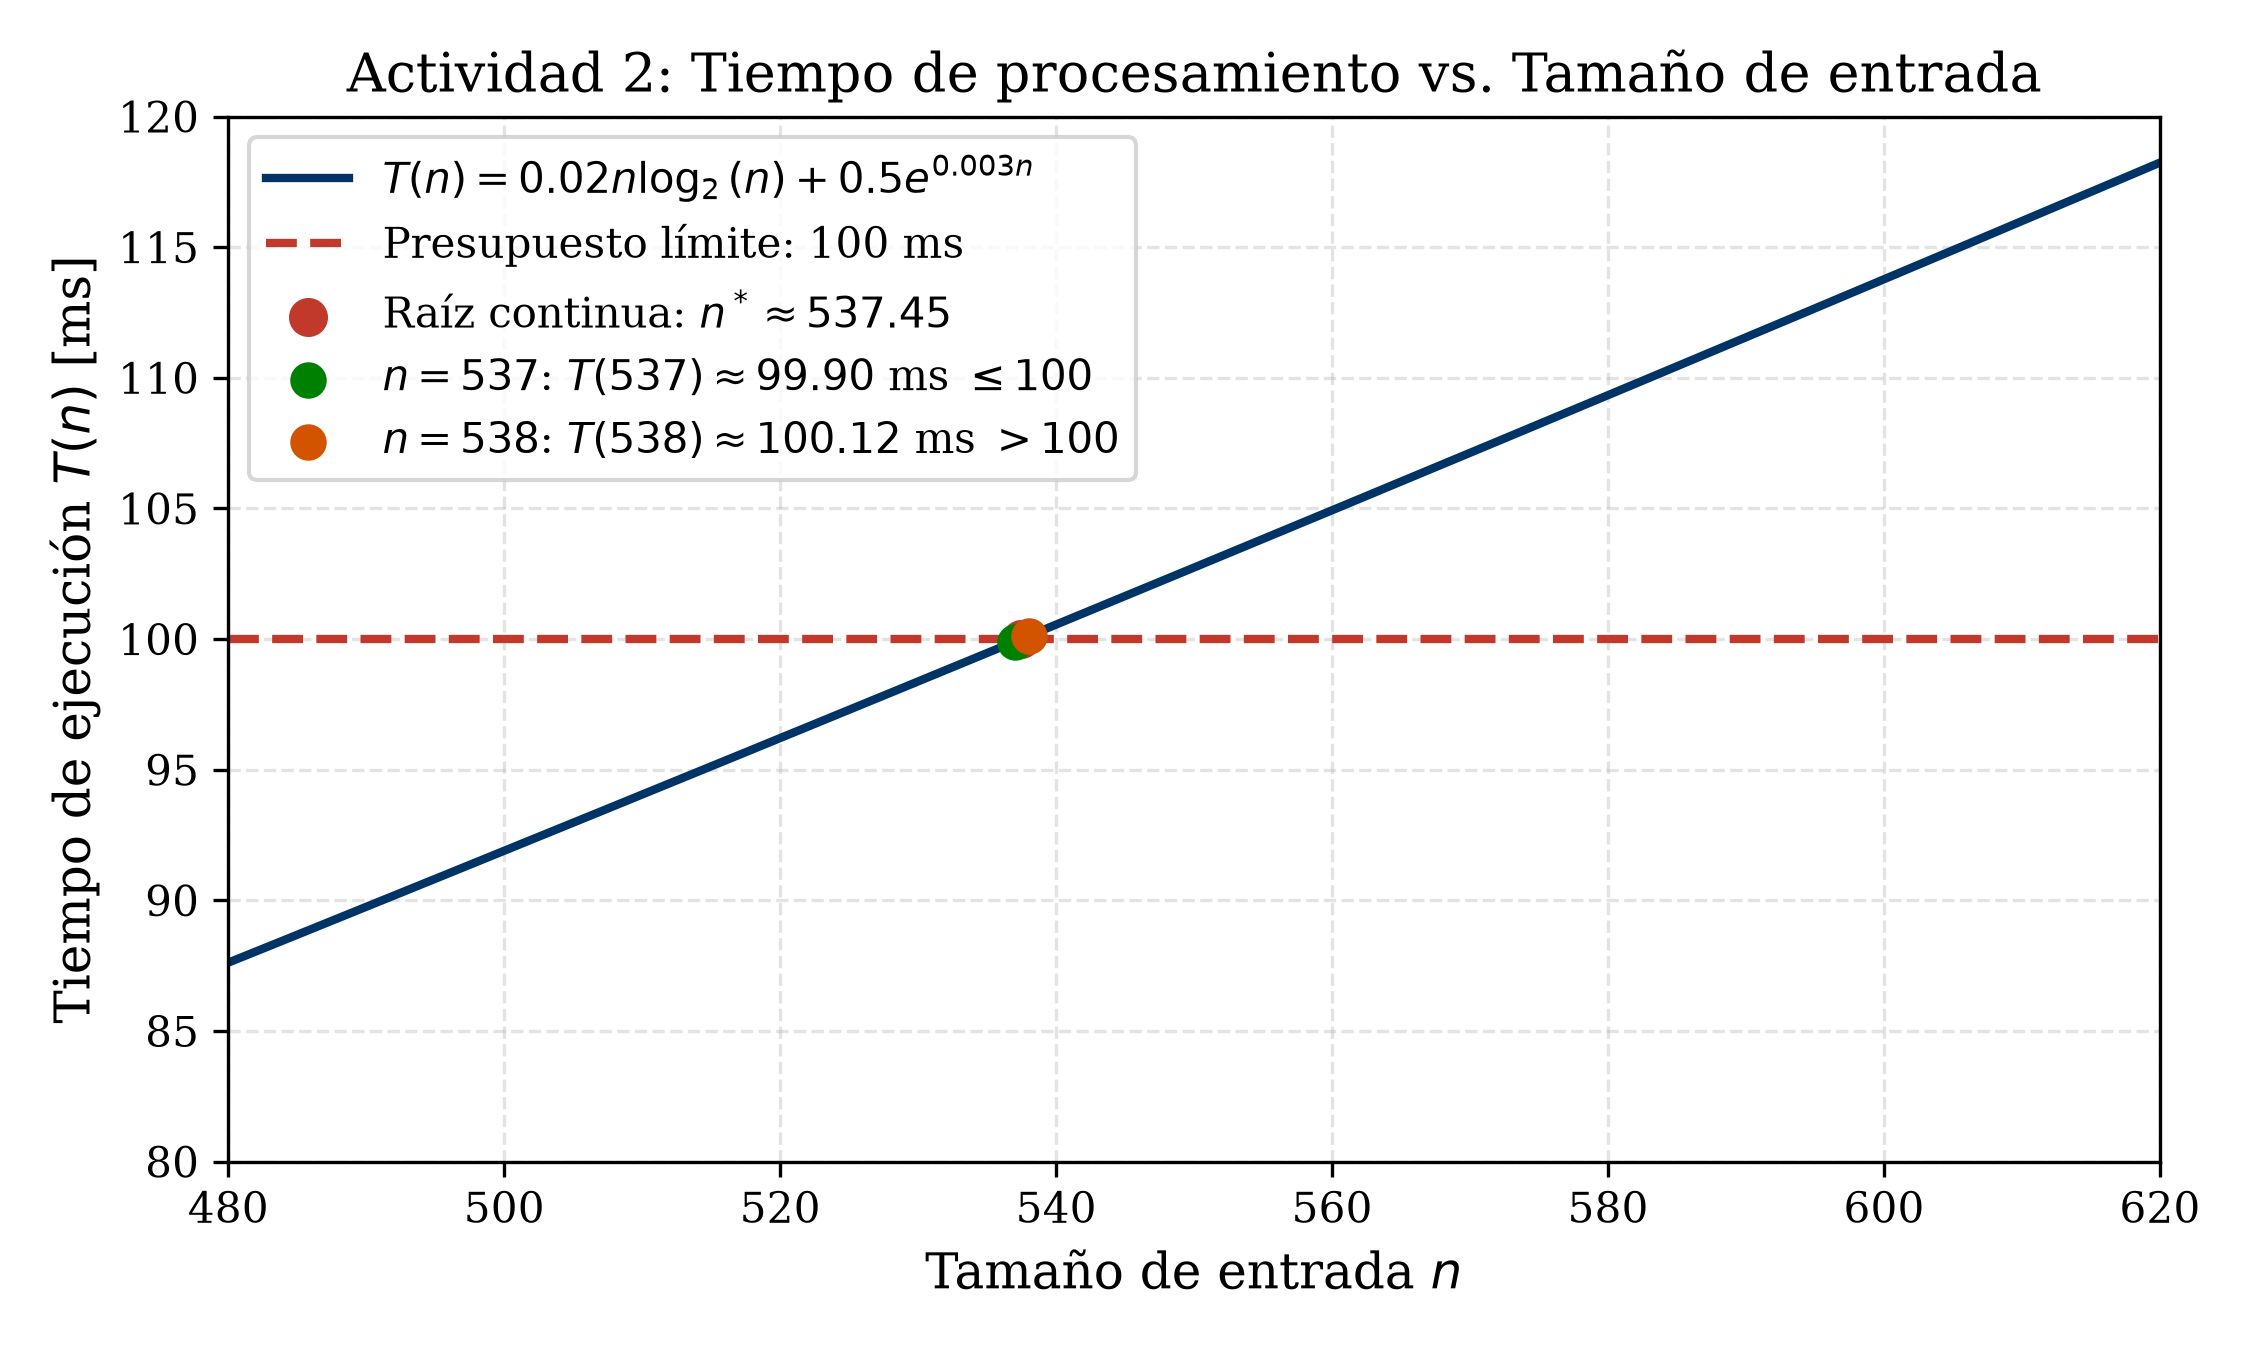
\includegraphics[width=0.72\textwidth]{fig_actividad2_tiempo_servicio.png}
    \caption{Tiempo de ejecución $T(n)$, límite de 100 ms y enteros cercanos a la raíz.}
\end{figure}

% ==============================================================================
% COMPARACIÓN DE RESULTADOS
% ==============================================================================
\section{Métodos y comparación de resultados}

\subsection{Descripción de los experimentos}
Para cada uno de los dos problemas se aplicaron los cinco métodos numéricos: bisección, Newton-Raphson, secante, falsa posición y punto fijo, utilizando las tolerancias $\varepsilon \in \{10^{-2}, 10^{-4}, 10^{-6}, 10^{-8}, 10^{-10}\}$.

En bisección el criterio de parada fue $\frac{b-a}{2} < \varepsilon$, y en los demás métodos fue $|x_{k+1} - x_k| < \varepsilon$. Para el método de punto fijo $x = g(x)$ se usaron las siguientes funciones:
\begin{itemize}[leftmargin=*]
    \item \textbf{Actividad 1:} $g(t) = t - \frac{f(t)}{16}$, que cumple $|g'(t^*)| = \left|1 - \frac{f'(t^*)}{16}\right| \approx 0.0033 < 1$.
    \item \textbf{Actividad 2:} $g(n) = n - f(n)$, que cumple $|g'(n^*)| = |1 - f'(n^*)| \approx 0.78 < 1$.
\end{itemize}

\subsection{Tablas comparativas}
Con la tolerancia más exigente ($\varepsilon = 10^{-10}$), los cinco métodos convergen al mismo resultado: $t^* \approx 5.3351058939$ y $n^* \approx 537.4473448160$. Las tablas muestran el número de iteraciones requerido en cada caso:

\begin{table}[h!]
    \centering
    \caption{Actividad 1: Número de iteraciones por método y tolerancia.}
    \label{tab:act1}
    \begin{tabular}{lccccc}
        \toprule
        Método & $10^{-2}$ & $10^{-4}$ & $10^{-6}$ & $10^{-8}$ & $10^{-10}$ \\
        \midrule
        Bisección       & $6$ & $13$ & $19$ & $26$ & $33$ \\
        Newton-Raphson  & $3$ & $4$  & $4$  & $4$  & $5$  \\
        Secante         & $3$ & $4$  & $5$  & $6$  & $6$  \\
        Falsa posición  & $3$ & $6$  & $8$  & $10$ & $12$ \\
        Punto fijo      & $3$ & $4$  & $4$  & $5$  & $6$  \\
        \bottomrule
    \end{tabular}
\end{table}

\begin{table}[h!]
    \centering
    \caption{Actividad 2: Número de iteraciones por método y tolerancia.}
    \label{tab:act2}
    \begin{tabular}{lccccc}
        \toprule
        Método & $10^{-2}$ & $10^{-4}$ & $10^{-6}$ & $10^{-8}$ & $10^{-10}$ \\
        \midrule
        Bisección       & $13$ & $19$ & $26$ & $33$ & $39$ \\
        Newton-Raphson  & $3$  & $3$  & $4$  & $4$  & $4$  \\
        Secante         & $3$  & $4$  & $4$  & $5$  & $5$  \\
        Falsa posición  & $3$  & $4$  & $5$  & $6$  & $7$  \\
        Punto fijo      & $29$ & $48$ & $66$ & $85$ & $104$ \\
        \bottomrule
    \end{tabular}
\end{table}

\begin{figure}[h!]
    \centering
    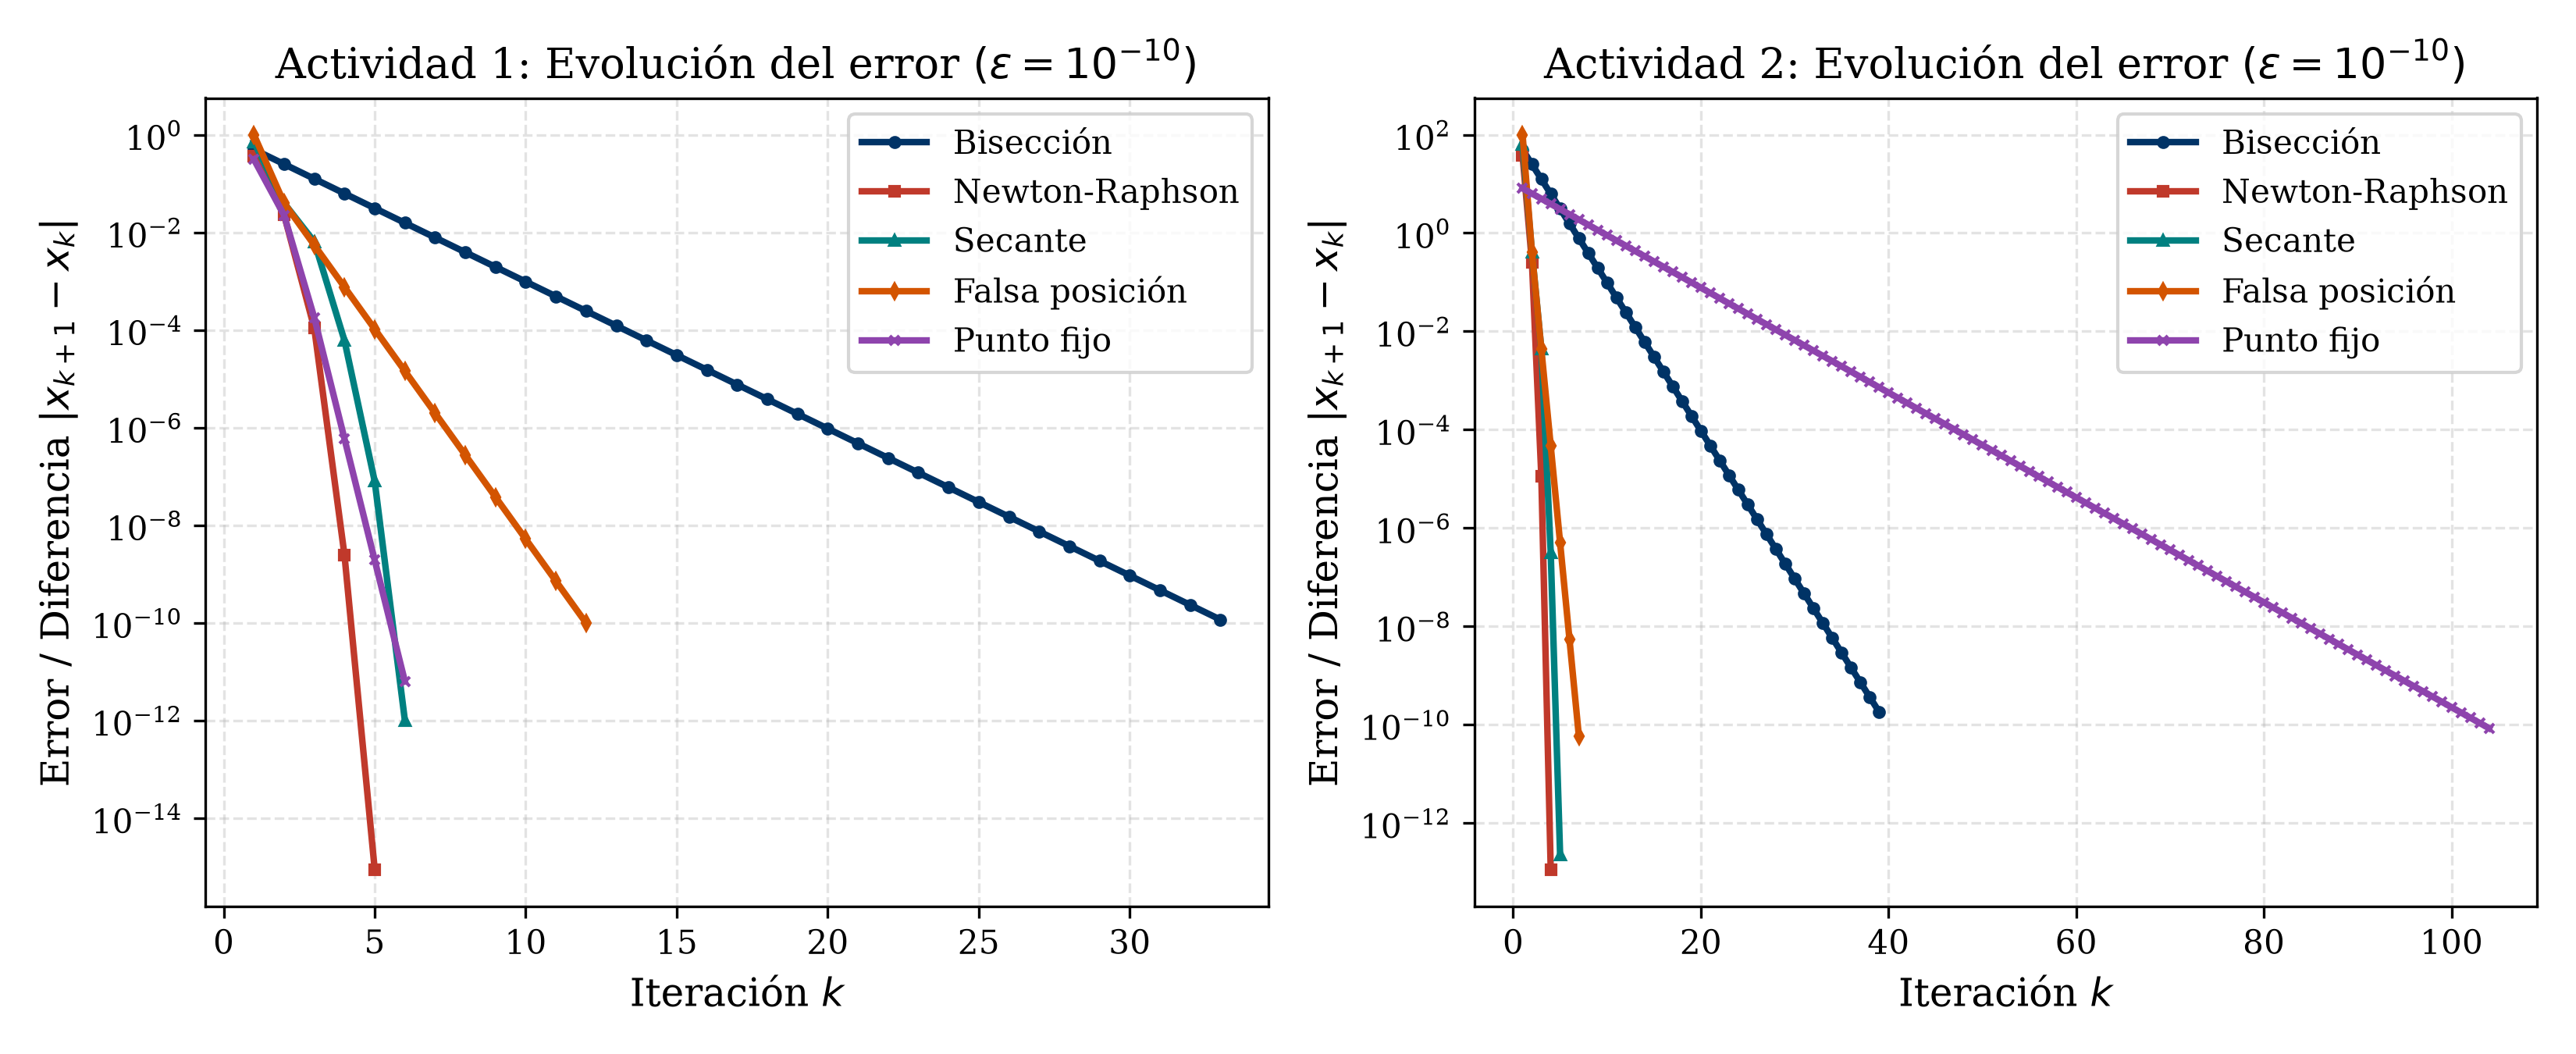
\includegraphics[width=0.92\textwidth]{fig_comparacion_convergencia.png}
    \caption{Disminución del error $|x_{k+1} - x_k|$ en función de las iteraciones ($\varepsilon = 10^{-10}$).}
\end{figure}

\subsection{Análisis de resultados}

\paragraph{Bisección:}
Fue el método que más iteraciones necesitó en la actividad 1 y el segundo en la actividad 2. Su comportamiento es completamente predecible: cada vez que la tolerancia baja en dos órdenes de magnitud ($10^{-2}$), necesita unas 6 o 7 iteraciones más, pues $\log_2(100) \approx 6.64$. Además, en la actividad 2 requiere más iteraciones que en la 1 porque el intervalo mide 100 en lugar de 1, lo que agrega unas $\log_2(100) \approx 6.6$ iteraciones fijas. Su ventaja principal es que siempre converge y garantiza una cota del error en todo momento.

\paragraph{Newton-Raphson:}
Fue el más rápido en ambos problemas. Pasar de $\varepsilon = 10^{-2}$ a $\varepsilon = 10^{-10}$ solo le tomó una o dos iteraciones más (de 3 a 5 en la actividad 1 y de 3 a 4 en la actividad 2). Esto refleja su convergencia cuadrática, donde la cantidad de cifras correctas casi se duplica en cada paso. Su desventaja práctica es que requiere calcular analíticamente la derivada $f'(x)$ y evaluarla junto con la función en cada iteración.

\paragraph{Secante:}
Tuvo un desempeño muy cercano a Newton, necesitando apenas una iteración más en la mayoría de los casos. Su orden de convergencia es superlineal ($\approx 1.618$). La gran ventaja es que no necesita calcular la derivada y solo evalúa la función una vez por iteración, lo que suele hacerlo computacionalmente más eficiente en la práctica.

\paragraph{Falsa posición:}
Comienza igual que la secante, pero al exigir más precisión se va quedando atrás: en la actividad 1 pasa de 3 a 12 iteraciones. Esto ocurre porque la función es convexa ($f''(t) > 0$), lo que hace que la recta secante siempre corte por debajo de la raíz; como resultado, el extremo derecho $b=6$ nunca se actualiza y el método pierde velocidad. En la actividad 2 la función es casi una recta en $[500, 600]$, por lo que este efecto casi no se nota y converge en 7 iteraciones.

\paragraph{Punto fijo:}
Mostró comportamientos muy diferentes en cada problema. En la actividad 1 convergió muy rápido (3 a 6 iteraciones) porque $|g'(t^*)| \approx 0.0033$, reduciendo el error a menos del $1\%$ en cada paso. En cambio, en la actividad 2 fue el más lento (hasta 104 iteraciones) porque $|g'(n^*)| \approx 0.78$, reduciendo el error solo al $78\%$ de la iteración anterior. Para ganar dos cifras decimales se necesitan unas $\frac{\ln(0.01)}{\ln(0.78)} \approx 19$ iteraciones, que coincide exactamente con los saltos observados en la tabla ($29 \to 48 \to 66 \to 85 \to 104$). Esto muestra que la velocidad de punto fijo depende totalmente de cómo se despeje la función $g(x)$.

\subsection{Comparación general}

\begin{table}[h!]
    \centering
    \caption{Resumen comparativo de los métodos.}
    \begin{tabular}{lcccc}
        \toprule
        Método & Convergencia & Requiere derivada & Raíz encerrada & Tipo \\
        \midrule
        Bisección       & Lineal & No & Sí & Cerrado \\
        Newton-Raphson  & Cuadrática & Sí & No & Abierto \\
        Secante         & Superlineal & No & No & Abierto \\
        Falsa posición  & Variable (lineal) & No & Sí & Cerrado \\
        Punto fijo      & Lineal (depende de $g$) & No & No & Abierto \\
        \bottomrule
    \end{tabular}
\end{table}

\paragraph{Conclusiones:}
\begin{itemize}[leftmargin=*]
    \item Los métodos cerrados (bisección y falsa posición) son más lentos pero seguros, ya que nunca se salen del intervalo.
    \item Los métodos abiertos (Newton y secante) convergen mucho más rápido cuando se tiene un buen valor inicial. Entre ellos, la secante resulta muy práctica porque no necesita la derivada analítica.
    \item En aplicaciones de ingeniería, no siempre es necesario buscar tolerancias extremas. En la actividad 2, como la respuesta final debe ser un número entero, una tolerancia de $\varepsilon = 10^{-2}$ ya fue suficiente para determinar que el tamaño máximo es $n_{\max} = 537$.
\end{itemize}

\end{document}
